\documentclass{article}
\usepackage[top=1in, bottom=1in, left=1in, right=1in]{geometry}
% \usepackage{fullpage, fancyhdr}
\usepackage{fullpage}
\usepackage{float}
\usepackage{mathtools}
\usepackage{xfrac}
\usepackage{graphicx}
\usepackage{caption}
\usepackage{subcaption}
\usepackage{portland}
%\usepackage{setspace}
\setlength{\topmargin}{0.0in}
\setlength{\headheight}{0.5in}
\setlength{\headsep}{0in}
\setlength{\footskip}{9pt}
\usepackage{listings}
\usepackage{color}

\usepackage{multicol}

\renewcommand{\arraystretch}{1.5}

\newcommand{\Lagr}{\mathcal{L}}

% For circuitikz
\usepackage[american,arrowmos]{circuitikz}
\usepackage{tikz}
\usetikzlibrary{calc}
\usepackage{pgfplots}
\usepackage{amsfonts}
\usetikzlibrary{shapes,arrows}

% \pagestyle{fancyplain}
\pagestyle{myheadings}
\voffset=-0.50in
\topmargin=0.00in 
\headsep=0.25in 
\evensidemargin=0in 
\oddsidemargin=0in 
\textwidth=6.6in 
\textheight=10.0in 

\renewcommand{\topfraction}{0.9}	% max fraction of floats at top
\renewcommand{\bottomfraction}{0.8}	% max fraction of floats at bottom
%   Parameters for TEXT pages (not float pages):
\setcounter{topnumber}{2}
\setcounter{bottomnumber}{2}
\setcounter{totalnumber}{4}     % 2 may work better
\setcounter{dbltopnumber}{2}    % for 2-column pages
\renewcommand{\dbltopfraction}{0.9}	% fit big float above 2-col. text
\renewcommand{\textfraction}{0.07}	% allow minimal text w. figs
%   Parameters for FLOAT pages (not text pages):
\renewcommand{\floatpagefraction}{0.7}	% require fuller float pages
% N.B.: floatpagefraction MUST be less than topfraction !!
\renewcommand{\dblfloatpagefraction}{0.7}	% require fuller float pages
% remember to use [htp] or [htpb] for placement

\title{Assignment \# 9: MEMS Gyroscope}
\date{4/17/2013}
\author{Brian Arnberg}

\markright{Brian Arnberg\hfill ELEC 6760 - Solid State Sensors\hfill}     
\setlength{\parindent}{0pt}


\begin{document}\label{start}

% \begin{titlepage}
% 	\maketitle
% 	\thispagestyle{empty}
% \end{titlepage}


\section*{ Homework Assignment \#9 - Due Wed. 4/17/13 }

A photograph of a MEMS gyroscope, that was fabricated in an SOI 
wafer, is presented in Figure~\ref{gyro}. The proof mass is 
forced to move along the x-axis and sensing is made along the 
y-axis. The z-axis is orthogonal to the photograph, i.e. out
of the paper. Answer the following questions about it:
\begin{figure}[h]
	\centering
	\vspace{-10pt}
	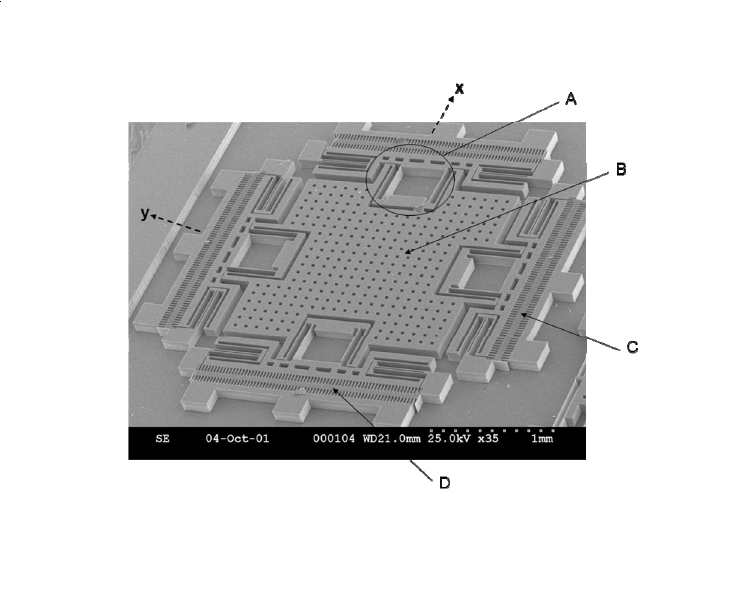
\includegraphics[keepaspectratio,width=0.75\textwidth]{gyro}
	\vspace{-40pt}
	\caption{MEMS Gyroscope on SOI wafer. Movement is in the x-axis, while sensing is in the y-axis.}
	\label{gyro}
	\vspace{-20pt}
\end{figure}

\renewcommand{\labelenumi}{\arabic{enumi})}

\begin{multicols}{2}
\begin{enumerate}
%--------------------------------------------------------------%
%---- Problem 1 -----------------------------------------------%
\item\label{p1}
What is ``A''?\\
\emph{
``A'' is part of the suspension system. 
}
	
%--------------------------------------------------------------%
%---- Problem 2 -----------------------------------------------%
\item\label{p2}
What is ``B''?\\
\emph{
``B'' is the proof mass.
}
  
%--------------------------------------------------------------%
%---- Problem 3 -----------------------------------------------%
\item\label{p3}
What are the holes in ``B'' for?\\	
\emph{
The holes in ``B'' are used for the release etching. 
}

%--------------------------------------------------------------%
%---- Problem 4 -----------------------------------------------%
\item\label{p4}
What is ``C'' and what is it used for?\\
\emph{
``C'' is a comb-drive actuator. It is used to actuate the proof
mass in the x-direction so that the system can detect motion in 
the y-direction.
}

%--------------------------------------------------------------%
%---- Problem 5 -----------------------------------------------%
\item\label{p5}
What is ``D'' and what is it used for?\\
\emph{
``D'' is an interdigitated sense capacitor circuit. It is used 
to detect movement in the y-direction.}

%--------------------------------------------------------------%
%---- Problem 6 -----------------------------------------------%
\item\label{p6}
About which axis would rotational motion be sensed with this 
gyroscope?\\
\emph{
Because the actuators are moving the mass along the x-axis, 
and because the gyroscope sensors detect motion in the y-axis, 
the gyroscope will sense  rotational motion about the 
z-axis. 
}

%--------------------------------------------------------------%
%---- Problem 7 -----------------------------------------------%
\item\label{p7}
Does this gyroscope sense angular position, angular rate, or 
angular acceleration?\\
\emph{
This gyroscope senses angular rate. 
}

%--------------------------------------------------------------%
%---- Problem 8 -----------------------------------------------%
\item\label{p8}
If the proof mass is 1$\mu g$, Q=100, $f_n$=10KHz, $A_x=1\mu N$, 
what is the damping coefficient, c, and the system spring 
constant, k, for the sensor?

\begin{tabular}{ l }
	$f_n = 10kHz \rightarrow \omega_n = 2 \pi 10 k rad/s$\\
	$\text{k }\colon {\omega_n}^2 = k / m \rightarrow k = {\omega_n}^2 m$\\
	$\text{  }\colon k = (2 \pi 10000 rad/s)^2 (1\times 10^{-9} kg)$\\
	$\text{  }\colon k = 3.948 N/m$\\
	$\text{c }\colon \omega_n / Q = c / m \rightarrow c = \frac{omega_n m}{Q}$\\
	$\text{  }\colon c = \frac{2 \pi 10000 rad/s \times 1\times10^{-9} kg}{100}$\\
	$\text{  }\colon c = 628.3 \times 10^{-9} N s /m$
\end{tabular}

%--------------------------------------------------------------%
%---- Problem 9 -----------------------------------------------%
\item\label{p9}
For the parameters in (\ref{p8}), what is the amplitude of 
displacement along the y-axis for $\Omega = 300^{\circ}/s$?

\begin{tabular}{ l }
	$\Omega = 300^{\circ}/s = 5.236 rad/s$\\
	$Y_d = \frac{2 m \Omega A_x}{c^2 \omega_n}$\\
	$\text{  }= \frac{2 (1\times10^{-9}) (5.236 rad/s) (1\times 10^{-6} N)}
		{(628.3\times 10^{-9} N s /m)^2 (2 \pi 10000 rad/s)}$\\
	$\text{  }= 422.25 \times 10^{-9} m$\\
	$Y_d = 422.25 nm$
\end{tabular}

%--------------------------------------------------------------%
%---- Problem 10 ----------------------------------------------%
\item\label{p10}
For the parameters in (\ref{p8}), what angular rate (in 
$^{\circ}$/s), results in an amplitude of displacement along the
y-axis of $1\mu m$?

\begin{tabular}{ l }
	$Y_d = \frac{2 m \Omega A_x}{c^2 \omega_n} \rightarrow
		\Omega = \frac{Y_d c^2 \omega_n}{2 m A_x}$\\
	$\Omega = \frac{(1\times10^{-6}m)(628.3 \times 10^{-9}N s/m)^2(2\pi 10000 rad/s)}
		{2 (1\times19^{-9} kg)(1\times10^{-6}N)}$\\
	$\Omega = 12.4 rad/s \rightarrow \Omega = 710.5^{\circ}/s$
\end{tabular}

%----- End Enumerate ------------------------------------------%
\end{enumerate}
%----- End Columns --------------------------------------------%
\end{multicols}

%--------------------------------------------------------------%
%---- Bottom of the page Figure -------------------------------%

\label{end}\end{document}


